% !TEX root = ../thesis_main.tex
\chapter{Ultrafast All-Optical Switching Based on the Optical Stark Effect in (6,5) SWCNTs}

\section{Introduction}


%{\color{red} UNFINISHED} %Talking about ultrafast optical switching. SWCNTs quite suited to this due to fast carrier dynamics, unlike those of inorganic semicondutors \cite{maeda2006gigantic}. Useful for optical switching processes such as those induced by the optical Stark effect. However, multi-photon processes occur that lead to the creation of real carriers which can photo-bleach the $E_{11}$ resonance if enough carriers are created and thereby limit the performance of the optical switching.

In this chapter, we present our observations of the optical Stark effect in an ensemble of individually suspended (6,5) SWCNTs that were dispersed using sodium deoxycholate (DOC). Following the discussion from Section \ref{sec:optical_stark_effect}, the optical Stark effect can be harnessed for ultrafast all-optical switching applications. We can quantify the performance of optical switching by using the term reversibility to describe how noncoherent carrier relaxation affects the performance of optical switching. Here, reversibility is defined as
%
\begin{equation}
 	\text{Rev} = \dfrac{\Delta T_\text{peak} - \Delta T_\text{base}}{\Delta T_\text{peak}},
  \label{eq:kira_reversibility}
\end{equation}
%
which includes the baseline transmission $\Delta T_\text{base}$ that represents the average of the transmission before and after switching occurs as well as the peak change in transmission $\Delta T_\text{peak}$, which only measures the coherent changes in transmission due to the optical Stark effect \cite{mack2019}. Furthermore, $\Delta T_\text{base}$ accounts for changes in transmission due to the creation of carriers via multiphoton processes. It also implicitly depends on other parameters such as the detuning and fluence of the optical pump as well as the time delay between incident pump pulses. The more that the optical pump is detuned below the $E_{11}$ resonance, the less likely that real excitons will be created through multiphoton excitations. Moreover, the time between successive pump pulses as well as the time scale of carrier relaxation can decay the reversibility of the system if carriers in the system accumulate over time after the arrival of consecutive pump pulses.

This chapter also features numerical simulations conducted by Professor Mackillo Kira and his PhD student Weiwei Jiang of the Electrical Engineering and Computer Science Department at the University of Michigan \cite{mack2019}. They solve Maxwell-semiconductor Bloch equations \cite{kira2011semiconductor, hirtschulz2008carbon} in a self-consistent manner for (6,5) SWCNTs. The semiconductor Bloch equations are given by
%
\begin{equation}
	\begin{split}
	i \hbar \frac{\partial}{\partial t} P_\text{k} &= \tilde{E}_\text{k} P_\text{k} - ( 1- f^\text{e}_\text{k} - f^\text{h}_\text{k})\Omega_\text{k} + \Gamma_\text{k}, \\
	\hbar \frac{\partial }{\partial t} f_\text{k}^\text{e(h)} &= 2 \text{Im}[P_\text{k}\Omega_\text{k}^*] + \Gamma^\text{e(h)}_\text{k}
	\end{split}
\end{equation}
%
 In a typical scenario, the optical pump pulse creates an electron (hole) distribution $f_\text{k}^\text{e(h)}$, via multiphoton processes, as well as a coherent polarization $P_\text{k}$ at the carrier momentum $\hbar k$. The term $\Gamma_\text{k}$ accounts for the Coulomb interactions between the carrier distributions and the initial coherent polarization. Moreover, the variable $\tilde{E}_\text{k}$ defined as
%
\begin{equation}
	\tilde{E}_\text{k} = E_\text{k} - \sum_\text{k'} V_\text{k - k'} ( f_\text{k'}^\text{e} + f_\text{k'}^\text{h}),
\end{equation}
%
refers to the renormalized electron-hole energy. This includes the bangap energy $E_\text{k}$ as well as the Coulomb matrix element $V_\text{k}$. In addition, $\Omega_\text{k}$ refers to the renormalized Rabi energy given as
\begin{equation}
	\Omega_\text{k} = d_\text{k} \cos\theta E(t) + \sum_\text{k'} V_\text{k - k'} P_\text{k'},
\end{equation}
which includes the matrix dipole element $d_\text{k}$, the electric field of the optical pump $E$ and the angle $\theta$ between the polarization of $E$ and the dipole moment associated with $d_\text{k}$. In the computations, these semiconductor Bloch equations are coupled directly to Maxwell's equations.

These calculations also account for noncoherent processes to help describe the dephasing kinetics which may affect the reversibility of the optical switching dynamics. Shortly after the initial photoexcitation, $P_\text{k}$ begins to dephase due to scattering events within the $f_\text{k}^\text{e(h)}$ distribution as a result of Coulomb interactions. From a phenomenological perspective, this dephasing can be described by an instantenous decay
\begin{equation}
	\dfrac{\partial}{\partial t} P_\text{k}(t) \Big|_\text{instant} = -\gamma P_\text{k}(t),
\end{equation}
which is parametrized by a dephasing constant $\gamma$ that implicitly accounts for quantum-kinetic scattering \cite{smith2010extraction, kira2011semiconductor}. However, in using a more microscopic approach, the effects of quantum memory emerge and the dephasing dynamics can be instead described using the expression
%
\begin{equation}\label{eq:kira_phenom_dephase}
	\dfrac{\partial}{\partial t} P_\text{k}(t) \Big|_\text{Q. Memory} = -\gamma \int^{t}_{\infty} dt' \left[ \exp\left\{ - \frac{\small i}{ \small \hbar} \hat{\mathcal{H}}_\text{ex}(t-t') \right\} P(t') \right]_\text{k} \exp \left(- \frac{t-t'}{T_\text{QM}} \right).
\end{equation}
%
In this expression, the exponential term parametrized by the Hamiltonian $\hat{\mathcal{H}}_\text{ex}(t-t')$ propagates the excitonic polarization forward in time. This Hamiltonian is expressed as
%
\begin{equation}
	\left[ \hat{\mathcal{H}}_\text{ex} \right]_\text{k, K}= \delta_\text{k, K} \tilde{E_\text{k}} - (1 - f_\text{k}^\text{e} - f_\text{k}^\text{h}) V_\text{k-K},
  \label{eq:kira_quantum_dephase}
\end{equation}
%
and acts as an effective Hamiltonian for excitons in the system. The other more curious term $T_\text{QM}$ defines the duration of the quantum memory.

Conceptually, quantum memory refers to the use of light as a carrier of information and encoding this information into matter \cite{iakoupov2013efficient}. In this context, the information of the optical pump gets stored within $P_\text{k}$, and can be retrieved by measuring the transmission of the optical probe to detect the shift of the $E_{11}$ resonance. The timescale defined by $T_\text{QM}$ not only determines how long this information is retained in $P_\text{k}$ before dephasing occurs but also plays a role in the magnitude of the dephasing as shown in Equation \eqref{eq:kira_quantum_dephase}. Experimental data, which will be presented in the next section, suggests that for SWCNTs, $T_\text{QM} \approx $ 66 fs which sufficiently reduces dephasing and thereby improves the reversibility of the system.

\section{Experimental Results}

Figure \ref{fig:ose_color_map} presents experimental data of the optical Stark effect observed in the (6,5)-enriched SWCNT suspension. The optical pump was negatively detuned below the $E_{11}$ resonance by $\sim 200$ meV and had a power density of 3.1 GW/cm$^2$. Figures \ref{fig:ose_dtt} and \ref{fig:ose_time_traces} complement this plot. Specifically, Figure \ref{fig:ose_dtt} shows the differential transmission probed at the $E_{11}$ transition energy, whereas Figure $\ref{fig:ose_time_traces}$ shows the attenuance spectrum before, during, and after the photo-excitation of the optical pump. Here, a coherent blueshift occurred at 0 fs.

Figure \ref{fig:ose_kira_nonresonant} shows more experimental data accompanied with numerical simulations. The data here was also collected using an optical pump detuned from the $E_{11}$ transition energy by $\sim$200 meV. Furthermore, the simulations compare how the coherent dynamics evolve both with and without the effects of quantum memory. The plot also shows how the Stark shift scales with the intensity of the optical pump.

The dynamics observed after resonant excitation of the $E_{11}$ transition are shown in Figure \ref{fig:ose_kira_resonant} along with numerical simulations. In this scenario, a spectral splitting located at the $E_{11}$ resonance occurs at both negative and positive time delays. This splitting is also predicted by the numerical simulations when using an appropriate dephasing constant $\gamma$. A second calculation with a reduced dephasing constant $\gamma/2$ is also presented as a point of comparison.

An investigation of the reversibility in the system using simulations is presented in Figure \ref{fig:ose_kira_simul}. These show how the reversibility, quantified by Equation \eqref{eq:kira_reversibility}, evolves with successive optical pumping induced by pulses of 200 fs duration that are spaced apart in time by 1 ps. The pump pulses are assumed to be detuned such that the detuning far exceeds the Rabi energy of the system. Here, reversibility is calculated in two scenarios. One scenario shows the change in the reversibility over time using the dephasing constant $\gamma$ that reproduces the experimental results. The second scenario instead uses a dephasing constant of $\gamma/2$ features optical pump excitations whose intensities and detuning are twice that of the previous scenario.

\begin{figure}[ht]
  \centering
  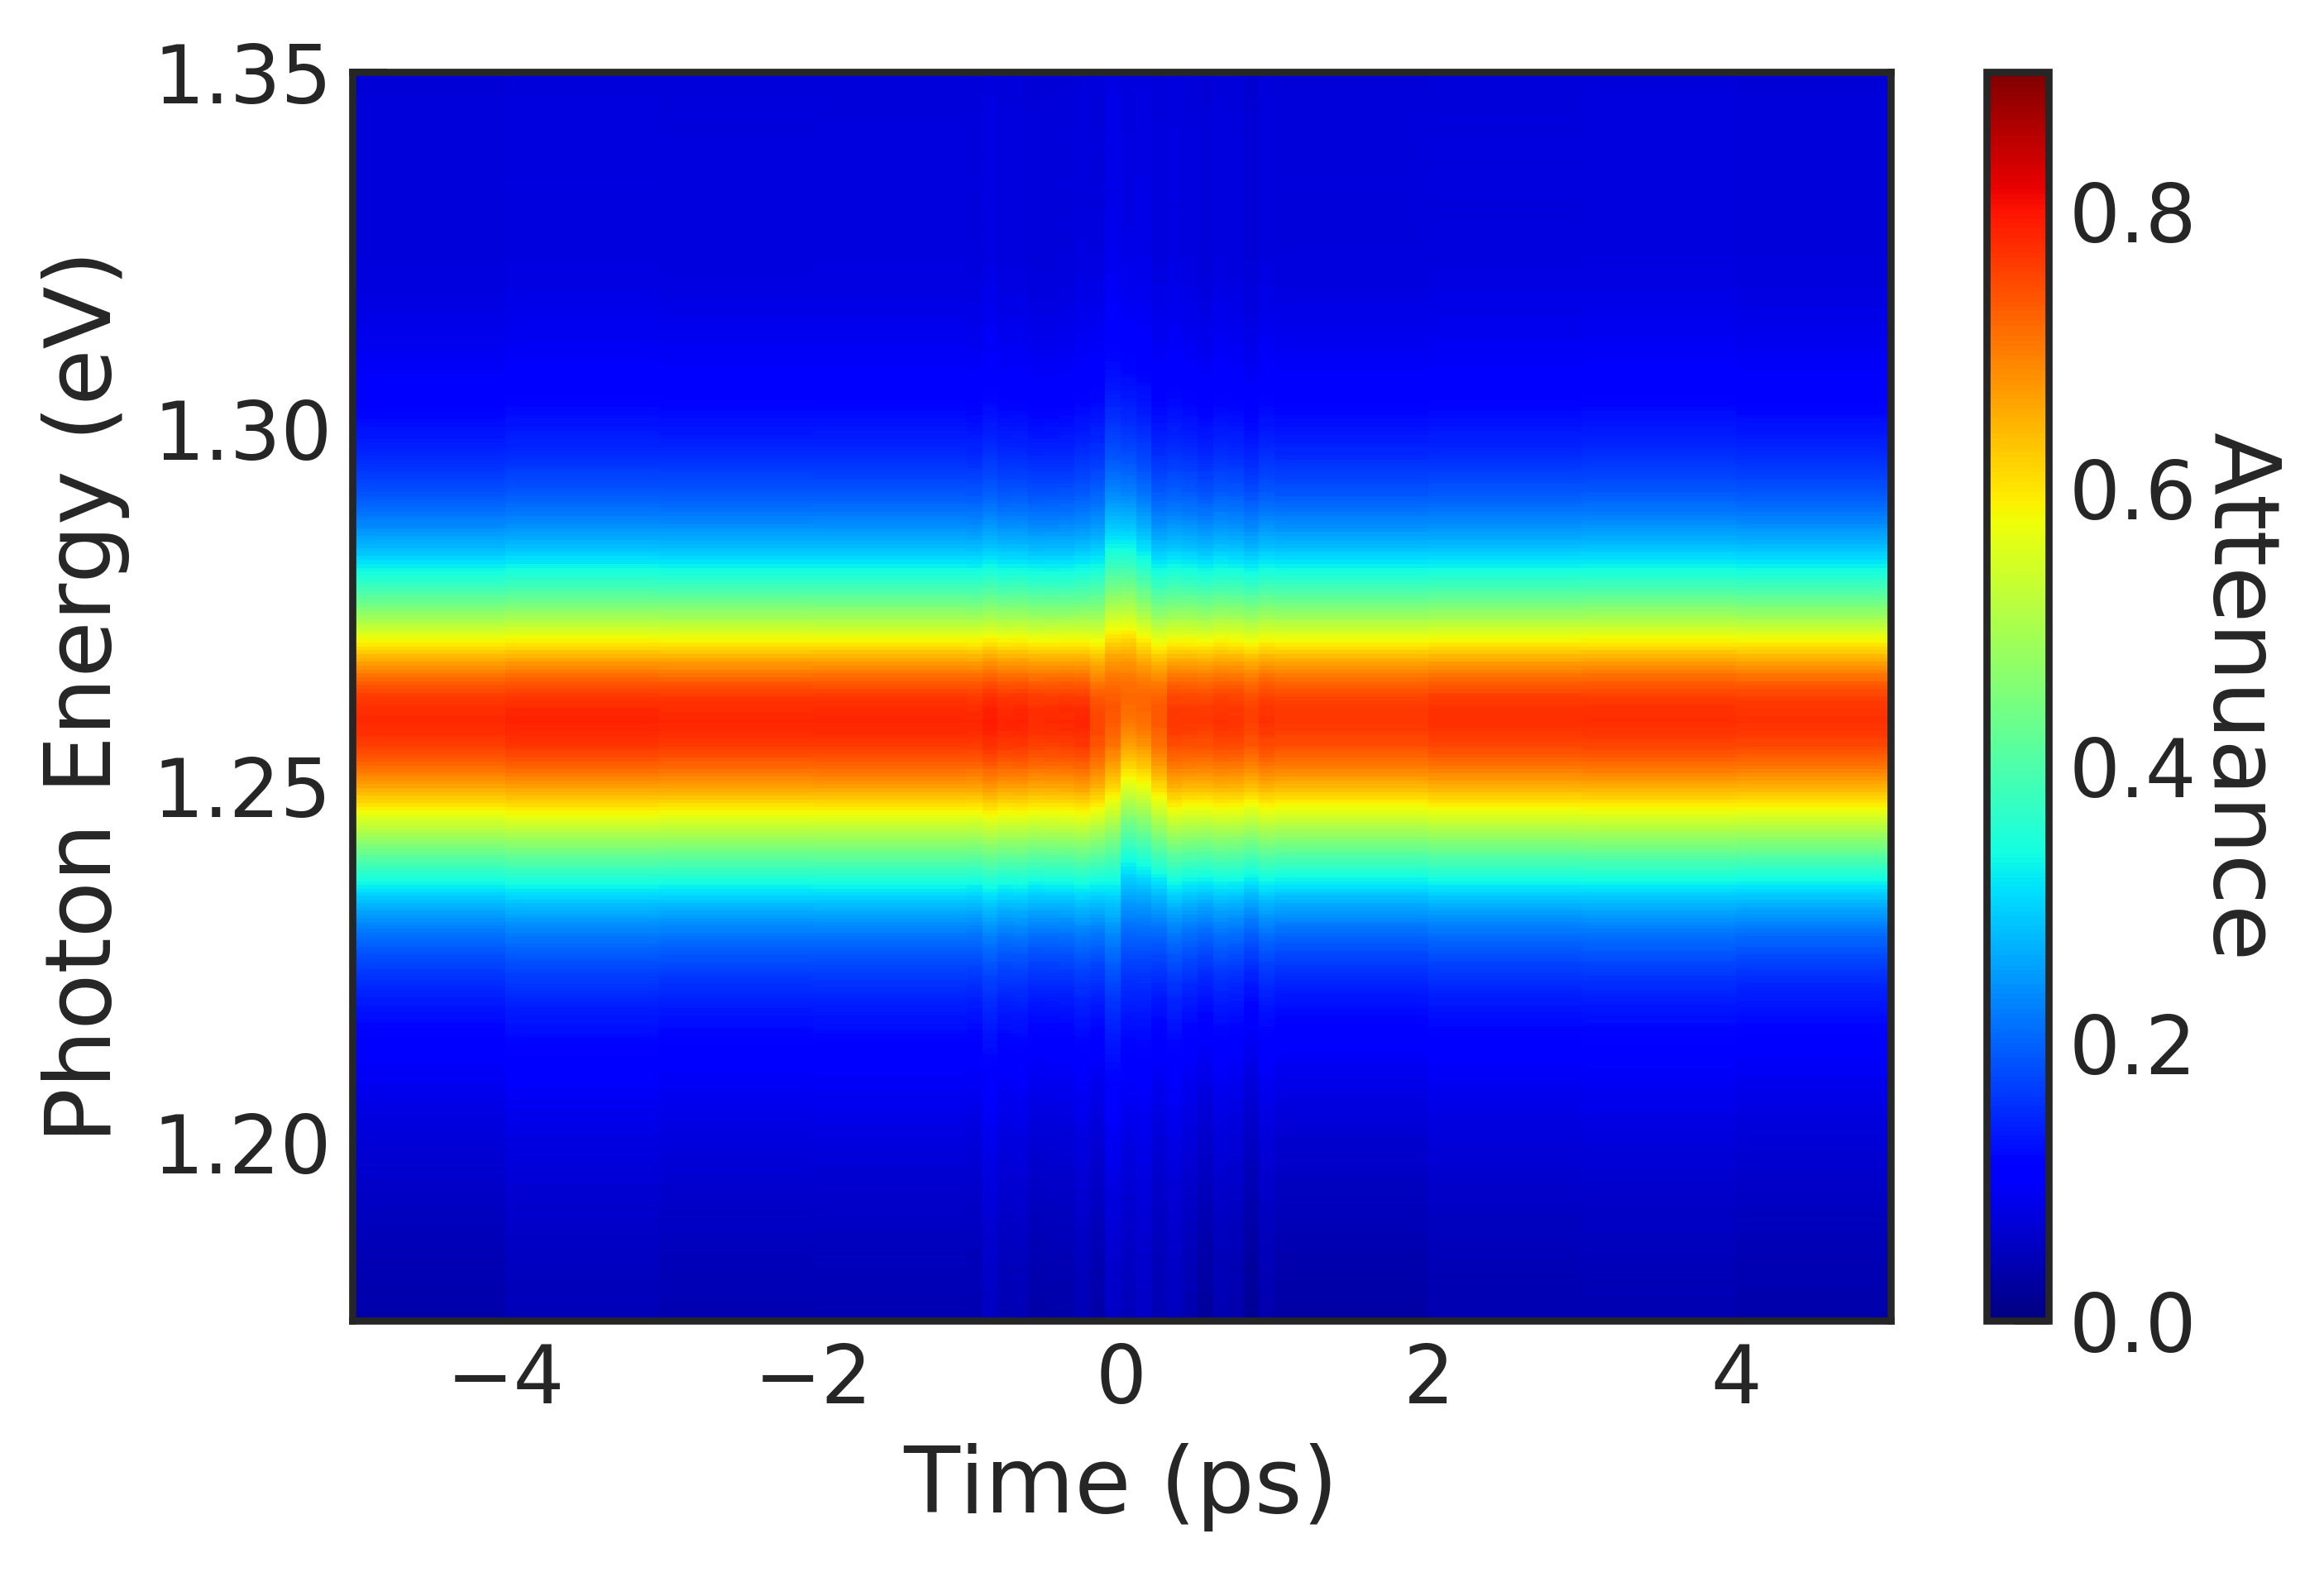
\includegraphics[height=2.4in]{images/chapter_coherent/ose_abs_map}
  \caption{ Color map of an optical Stark effect measurement of the $E_{11}$ resonance. Here, the optical pump photon energy is detuned by $\sim$200 meV relative to the $E_{11}$ transition energy and has a power density of 3.1 GW/cm$^2$. At a time delay of 0 ps, $E_{11}$ resonance shifts by 3 meV. This shift quickly disappears at later time delays. }
  \label{fig:ose_color_map}
\end{figure}

\begin{figure}[ht]
  \centering
  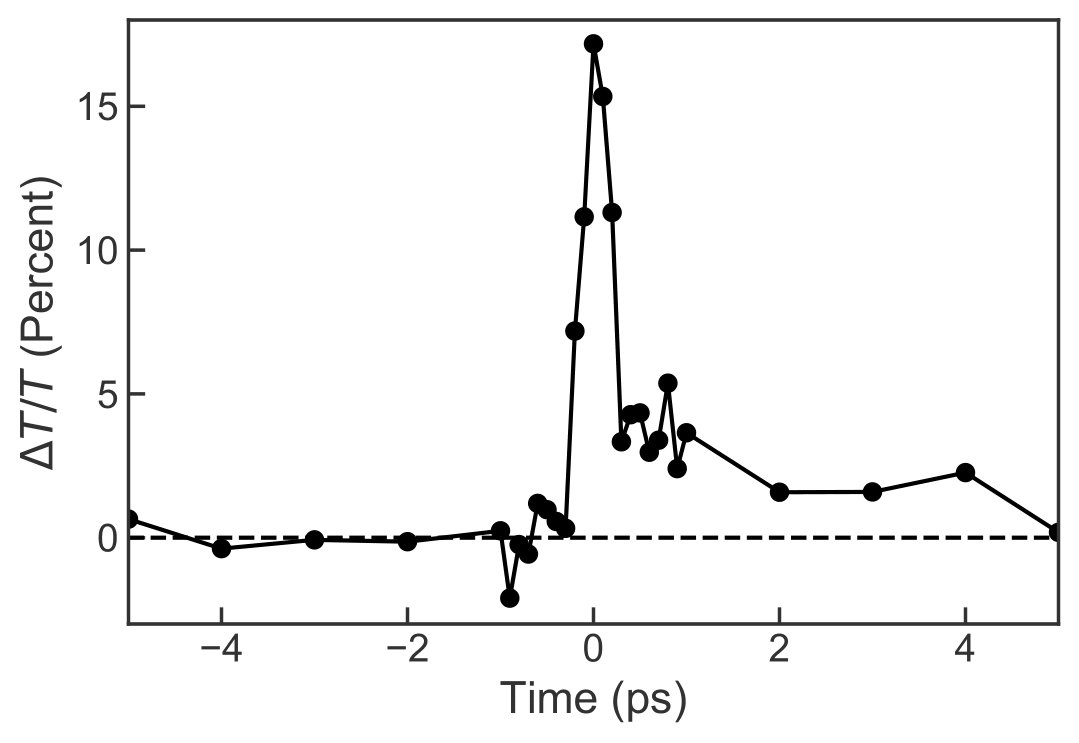
\includegraphics[height=2.4in]{images/chapter_coherent/ose_dt}
  \caption{Differential transmission probed at the $E_{11}$ resonance from the data shown in Figure \ref{fig:ose_color_map}. A large signal originating from the optical Stark effect occurs at the time delay of 0 ps. The remaining signal at later delays emerges due to the creation of excitons via multiphoton processes. }
  \label{fig:ose_dtt}
\end{figure}

\begin{figure}[ht]
  \centering
  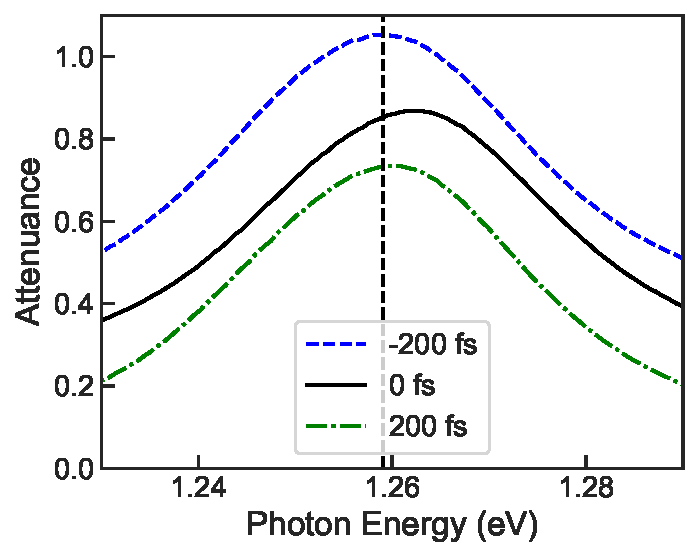
\includegraphics[height=2.4in]{images/chapter_coherent/ose_time_traces}
  \caption{$E_{11}$ attenuance spectrum as a function of time. The data shown here correspond to vertical slices of the plot shown in Figure \ref{fig:ose_color_map}. The $E_{11}$ peak shifts coherently at 0 ps due to the optical Stark effect. At slightly earlier and later time delays, this shift does not occur. Each curve has been  manually offset for clarity.}
  \label{fig:ose_time_traces}
\end{figure}

\begin{figure}[ht]
	\centering
	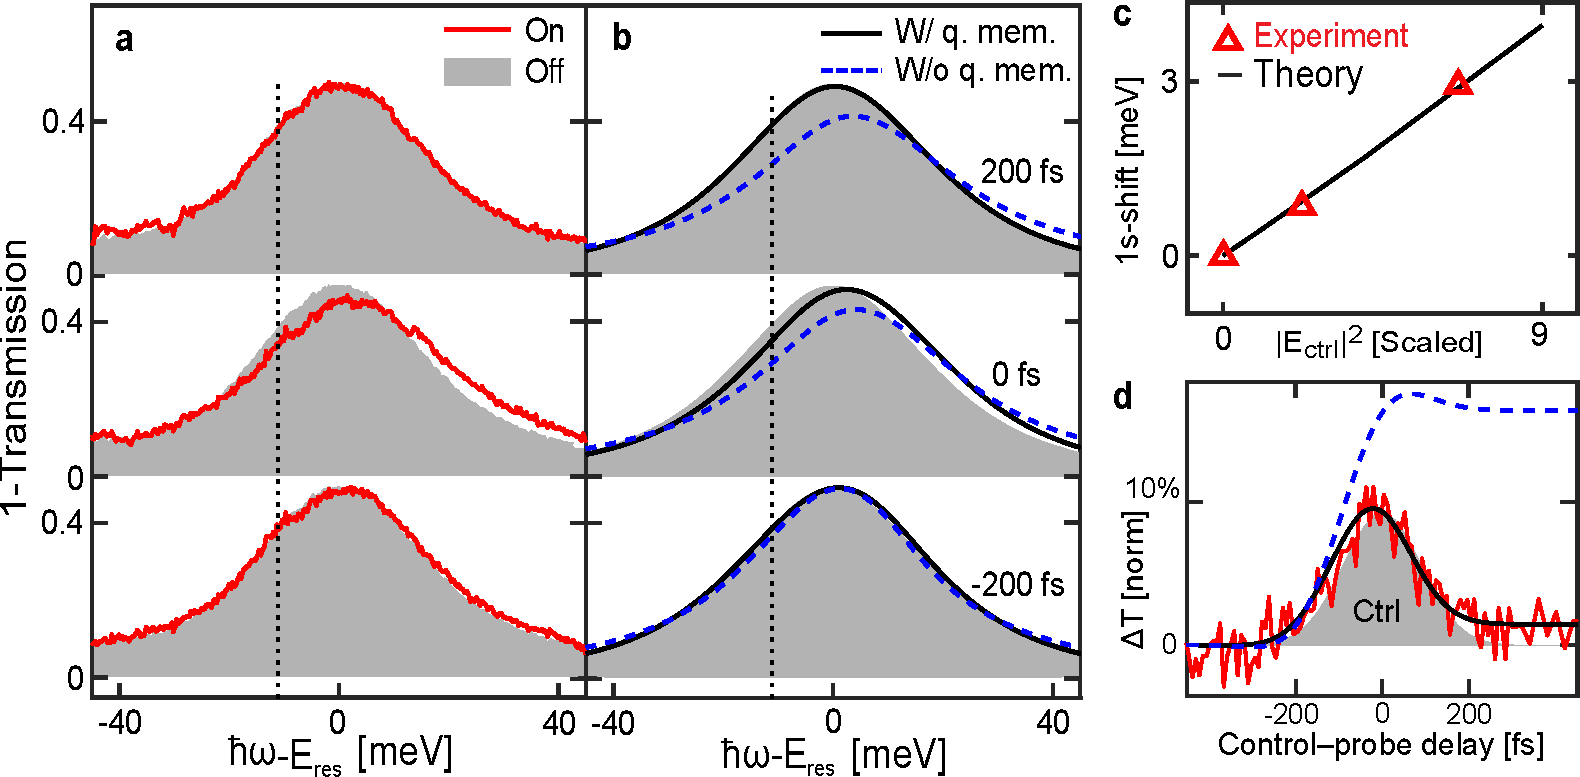
\includegraphics[height=2.6in]{images/chapter_coherent/nonresonant}
	\caption{(a) Measured vs.\ (b) numerically simulated transmission spectra of the SWCNT ensemble both with (solid lines) and without (shaded area) the influence of the optical pump beam. Here, the optical pump photon energy is detuned by 200 meV relative to the $E_{11}$ resonance. The dashed line shows how the transmission spectrum would evolve by using the phenomenological description of the dephasing dynamics represented in Equation \eqref{eq:kira_phenom_dephase} as opposed to the quantum-kinetic approach given by Equation \eqref{eq:kira_quantum_dephase}. Without considering quantum memory, the $E_{11}$ resonance becomes slightly photobleached and shifts in a noncoherent fashion. However, the quantum-kinetic description that includes quantum memory agrees with the experimental data. (c) Calculated (solid line) vs. experimentally measured Stark shift $\Delta E$. The Stark shift scales linearly with the intensity of the optical pump beam expressed as $|E_\text{ctrl}|^2$ (d) Time-resolved differential transmission probed at the $E_{11}$ resonance. The shaded area represent the temporal profile of the optical pump pulse. The curves correspond to experimental data (solid red line), a theoretical calculation including quantum memory (solid black line) and another computation excluding the effects of quantum memory (dashed blue line). Reproduced from Ref.\ \cite{mack2019}.}

  \label{fig:ose_kira_nonresonant}
\end{figure}

\begin{figure}[ht]
	\centering
	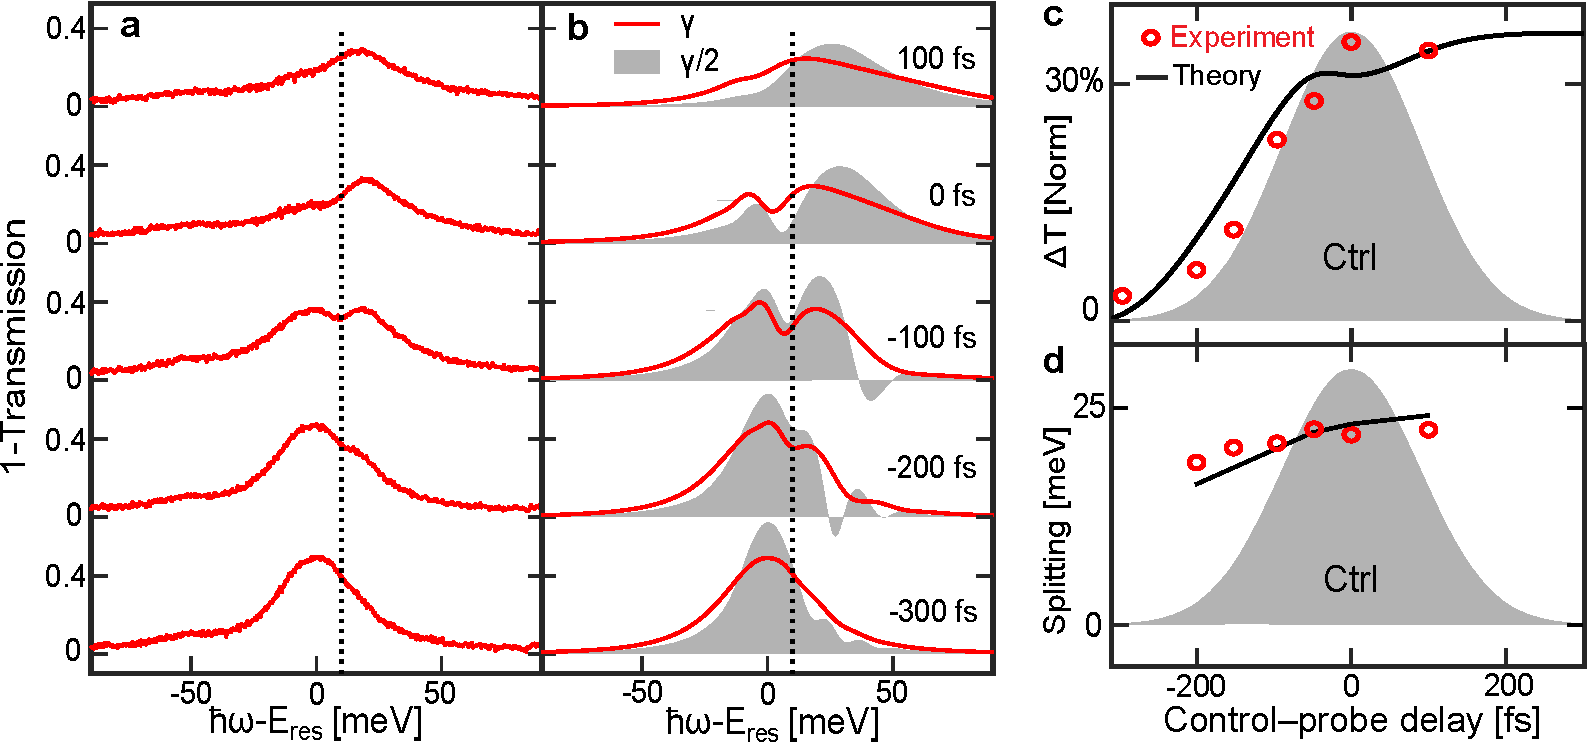
\includegraphics[height=2.6in]{images/chapter_coherent/resonant}
	\caption{(a) Experimental and (b) numerically simulated transmission for five pump-probe time delays with the optical pump photon energy equaling that of the $E_{11}$ transition. The shaded areas correspond to the computed transmission with the dephasing constant reduced by a factor of one-half. (c) Differential transmission and (d) energy splitting at the $E_{11}$ resonancs vs.\ pump-probe delay time. The shaded figures represent the temporal profile of the optical pump pulse. A spectral splitting occurs even at times before the arrival of the optical pump pulse. Reproduced from Ref.\ \cite{mack2019} }

  \label{fig:ose_kira_resonant}
\end{figure}


\begin{figure}[ht]
	\centering
	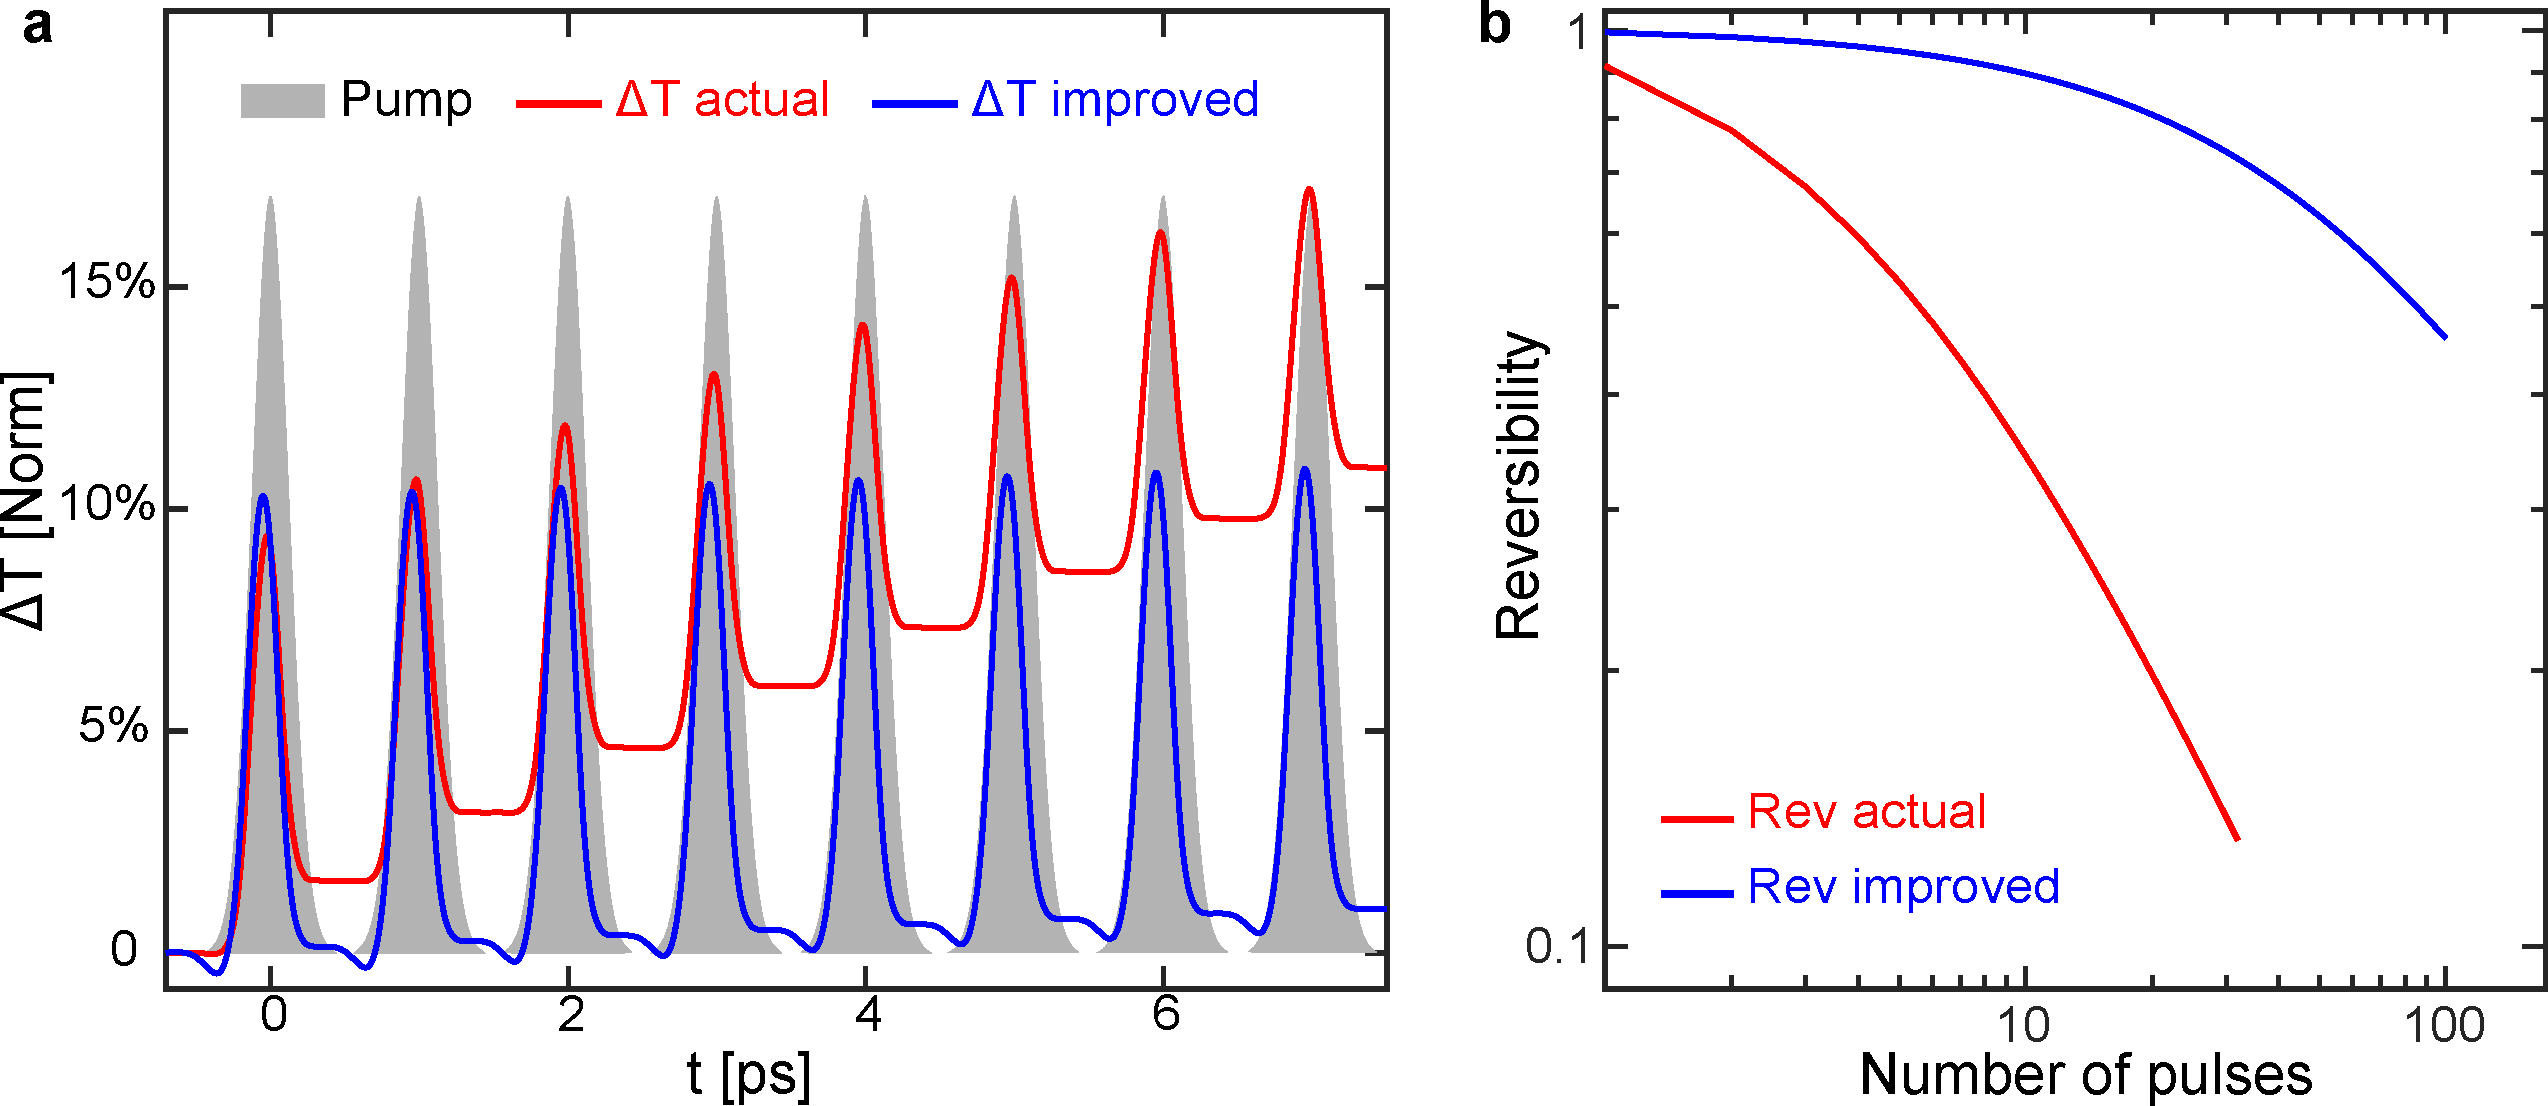
\includegraphics[height=2.6in]{images/chapter_coherent/switching_reversibility}
	\caption{ Simulation of ultrafast switching reversibility. (a) Calculated differential transmission within the span of eight 200 fs optical pulses irradiating the system. The pump pulses are detuned below the $E_{11}$ resonance such that the detuning is much greater than the Rabi energy. The shaded area represents temporal profile of the incident optical pump pulses. The red curves show predicted change in differential transmission over time of using desphasing parameter $\gamma$ that reproduces experimental data. The blue curve shows how the differential transmission changes using $\gamma/2$ as the new dephasing constant and doubling the detuning and the pump intensity. (b) Predicted reversibility of the SWCNT system using the definition established in Equation \eqref{eq:kira_reversibility}. The red and blue curves correspond to conditions defined in the red and blue curves shown in Figure (a) respectively.  Reproduced from Ref.\ \cite{mack2019}.}
  \label{fig:ose_kira_simul}
\end{figure}



\clearpage

\section{Discussion}

A clear signature of the optical Stark effect is observed in Figure \ref{fig:ose_color_map}. The change in the attenuance of the $E_{11}$ peak only occurs at a time delay of 0 ps. In Figure \ref{fig:ose_dtt}, a large change in the differential transmission also only occurs at 0 ps. The positive signal observed at later time delays is interpreted as a result of photobleaching due to real excitons created as a result of multiphoton processes. Furthermore, the energy shift of the $E_{11}$ resonance is clearly resolved in Figure \ref{fig:ose_time_traces} where at 0 ps the $E_{11}$ peak shifts by 3 meV. Otherwise, at times before and after the arrival of the optical pump pulse, the peak retains its original position.

Figures \ref{fig:ose_kira_nonresonant}(a) and \ref{fig:ose_kira_nonresonant}(b) demonstrate the necessity of invoking the effects of quantum memory to explain these results. In using the phenomenological approach captured by Equation \eqref{eq:kira_phenom_dephase}, the numerical simulations predict dynamics that do not agree with the experimental data. Under these conditions, the $E_{11}$ resonance irreversibly shifts, and retains this energy shift even at time delays after the arrival of the optical pump pulse. In contrast, the calculations incorporating the effects of quantum memory successfully reproduce the coherent shift of the $E_{11}$ transition.

In addition, Figure \ref{fig:ose_kira_nonresonant}(c) shows that the energy shift scales linearly with the intensity of the optical pump, a result which shows proper correspondence with the optical Stark effect. Figure \ref{fig:ose_kira_nonresonant}(d) shows how the differential transmission at the $E_{11}$ resonance changes with time delay. The experimental data as well as the numerical simulation including quantum memory both feature a significant coherent component that matches the temporal profile of the optical pump pulse. However, the calculations that exclude quantum memory show a marginally small coherent component that is instead dominated by incoherent effects due to the creation of real carriers.

The $E_{11}$ peak exhibits a spectral splitting when the optical pump photon energy equals that of the $E_{11}$ transition, as shown in Figure \ref{fig:ose_kira_resonant}. This splitting is also reproduced by numerical simulations that account for quantum memory. However, this splitting still occurs at both positive and negative time delays, as shown by Figure \ref{fig:ose_kira_resonant}(d). This alone shows that the energy splitting cannot indicate a Rabi splitting that is expected to occur with zero detuning. These are instead interpreted as coherent oscillations that occur due to wave-mixing between the optical pump and probe \cite{joffre1988coherent}. It is said that these two light beams, each with their own wave vectors, interfere and subsequently introduce spectral ringing to the optical probe \cite{joffre1988coherent}.

Figure \ref{fig:ose_kira_simul} employs numerical simulations to illustrate how reversibility changes after irradiating the system with successive optical pump pulses. In this scenario, the rate at which reversibility decreases depends on the accumulation of carriers via multiphoton processes after the arrival of each optical pump pulse. Hence, the relevant quantities of interest include the rate of carrier relaxation as well as the time delay between each consecutive pump pulse. The data show that the reversibility of the hypothetical sample with a dephasing constant of $\gamma/2$ diminishes 20 times slower than in the current sample. For the hypothetical sample, reversibility is found to be as high as 10\% after 500 optical pump pulses.

\section{Conclusions}

In conclusion, we have clearly resolved the optical Stark effect in a (6,5)-enriched SWCNT suspension. For ultrafast all-optical switching applications, using a pump detuned below the $E_{11}$ to excite the SWCNTs is preferable as a reversible energy shift of the $E_{11}$ transition occurs and any carriers created via multiphoton effects will decay on a picosecond timescale. These results are well explained by using a nonphenomenological theoretical approach that incorporates the effects of quantum memory. Without accounting for quantum memory, numerical calculations instead predict an irreversible shift due to instantaneous dephasing. In the case of resonant $E_{11}$ excitations, an irreversible process occurs due to spectral ringing of the probe beam which occurs as due to wave-mixing between the optical pump and probe. Finally, we observe that the reversibility of the system can be substantially improved by detuning the optical pump photon energy further below the $E_{11}$ resonance and using a sample with a lower dephasing constant.
